% Options for packages loaded elsewhere
\PassOptionsToPackage{unicode}{hyperref}
\PassOptionsToPackage{hyphens}{url}
%
\documentclass[
  11pt,
]{article}
\usepackage{amsmath,amssymb}
\usepackage{iftex}
\ifPDFTeX
  \usepackage[T1]{fontenc}
  \usepackage[utf8]{inputenc}
  \usepackage{textcomp} % provide euro and other symbols
\else % if luatex or xetex
  \usepackage{unicode-math} % this also loads fontspec
  \defaultfontfeatures{Scale=MatchLowercase}
  \defaultfontfeatures[\rmfamily]{Ligatures=TeX,Scale=1}
\fi
\usepackage[]{libertine}
\ifPDFTeX\else
  % xetex/luatex font selection
\fi
% Use upquote if available, for straight quotes in verbatim environments
\IfFileExists{upquote.sty}{\usepackage{upquote}}{}
\IfFileExists{microtype.sty}{% use microtype if available
  \usepackage[]{microtype}
  \UseMicrotypeSet[protrusion]{basicmath} % disable protrusion for tt fonts
}{}
\makeatletter
\@ifundefined{KOMAClassName}{% if non-KOMA class
  \IfFileExists{parskip.sty}{%
    \usepackage{parskip}
  }{% else
    \setlength{\parindent}{0pt}
    \setlength{\parskip}{6pt plus 2pt minus 1pt}}
}{% if KOMA class
  \KOMAoptions{parskip=half}}
\makeatother
\usepackage{xcolor}
\usepackage[margin=1in]{geometry}
\usepackage{color}
\usepackage{fancyvrb}
\newcommand{\VerbBar}{|}
\newcommand{\VERB}{\Verb[commandchars=\\\{\}]}
\DefineVerbatimEnvironment{Highlighting}{Verbatim}{commandchars=\\\{\}}
% Add ',fontsize=\small' for more characters per line
\usepackage{framed}
\definecolor{shadecolor}{RGB}{248,248,248}
\newenvironment{Shaded}{\begin{snugshade}}{\end{snugshade}}
\newcommand{\AlertTok}[1]{\textcolor[rgb]{0.94,0.16,0.16}{#1}}
\newcommand{\AnnotationTok}[1]{\textcolor[rgb]{0.56,0.35,0.01}{\textbf{\textit{#1}}}}
\newcommand{\AttributeTok}[1]{\textcolor[rgb]{0.13,0.29,0.53}{#1}}
\newcommand{\BaseNTok}[1]{\textcolor[rgb]{0.00,0.00,0.81}{#1}}
\newcommand{\BuiltInTok}[1]{#1}
\newcommand{\CharTok}[1]{\textcolor[rgb]{0.31,0.60,0.02}{#1}}
\newcommand{\CommentTok}[1]{\textcolor[rgb]{0.56,0.35,0.01}{\textit{#1}}}
\newcommand{\CommentVarTok}[1]{\textcolor[rgb]{0.56,0.35,0.01}{\textbf{\textit{#1}}}}
\newcommand{\ConstantTok}[1]{\textcolor[rgb]{0.56,0.35,0.01}{#1}}
\newcommand{\ControlFlowTok}[1]{\textcolor[rgb]{0.13,0.29,0.53}{\textbf{#1}}}
\newcommand{\DataTypeTok}[1]{\textcolor[rgb]{0.13,0.29,0.53}{#1}}
\newcommand{\DecValTok}[1]{\textcolor[rgb]{0.00,0.00,0.81}{#1}}
\newcommand{\DocumentationTok}[1]{\textcolor[rgb]{0.56,0.35,0.01}{\textbf{\textit{#1}}}}
\newcommand{\ErrorTok}[1]{\textcolor[rgb]{0.64,0.00,0.00}{\textbf{#1}}}
\newcommand{\ExtensionTok}[1]{#1}
\newcommand{\FloatTok}[1]{\textcolor[rgb]{0.00,0.00,0.81}{#1}}
\newcommand{\FunctionTok}[1]{\textcolor[rgb]{0.13,0.29,0.53}{\textbf{#1}}}
\newcommand{\ImportTok}[1]{#1}
\newcommand{\InformationTok}[1]{\textcolor[rgb]{0.56,0.35,0.01}{\textbf{\textit{#1}}}}
\newcommand{\KeywordTok}[1]{\textcolor[rgb]{0.13,0.29,0.53}{\textbf{#1}}}
\newcommand{\NormalTok}[1]{#1}
\newcommand{\OperatorTok}[1]{\textcolor[rgb]{0.81,0.36,0.00}{\textbf{#1}}}
\newcommand{\OtherTok}[1]{\textcolor[rgb]{0.56,0.35,0.01}{#1}}
\newcommand{\PreprocessorTok}[1]{\textcolor[rgb]{0.56,0.35,0.01}{\textit{#1}}}
\newcommand{\RegionMarkerTok}[1]{#1}
\newcommand{\SpecialCharTok}[1]{\textcolor[rgb]{0.81,0.36,0.00}{\textbf{#1}}}
\newcommand{\SpecialStringTok}[1]{\textcolor[rgb]{0.31,0.60,0.02}{#1}}
\newcommand{\StringTok}[1]{\textcolor[rgb]{0.31,0.60,0.02}{#1}}
\newcommand{\VariableTok}[1]{\textcolor[rgb]{0.00,0.00,0.00}{#1}}
\newcommand{\VerbatimStringTok}[1]{\textcolor[rgb]{0.31,0.60,0.02}{#1}}
\newcommand{\WarningTok}[1]{\textcolor[rgb]{0.56,0.35,0.01}{\textbf{\textit{#1}}}}
\usepackage{longtable,booktabs,array}
\usepackage{calc} % for calculating minipage widths
% Correct order of tables after \paragraph or \subparagraph
\usepackage{etoolbox}
\makeatletter
\patchcmd\longtable{\par}{\if@noskipsec\mbox{}\fi\par}{}{}
\makeatother
% Allow footnotes in longtable head/foot
\IfFileExists{footnotehyper.sty}{\usepackage{footnotehyper}}{\usepackage{footnote}}
\makesavenoteenv{longtable}
\usepackage{graphicx}
\makeatletter
\def\maxwidth{\ifdim\Gin@nat@width>\linewidth\linewidth\else\Gin@nat@width\fi}
\def\maxheight{\ifdim\Gin@nat@height>\textheight\textheight\else\Gin@nat@height\fi}
\makeatother
% Scale images if necessary, so that they will not overflow the page
% margins by default, and it is still possible to overwrite the defaults
% using explicit options in \includegraphics[width, height, ...]{}
\setkeys{Gin}{width=\maxwidth,height=\maxheight,keepaspectratio}
% Set default figure placement to htbp
\makeatletter
\def\fps@figure{htbp}
\makeatother
\setlength{\emergencystretch}{3em} % prevent overfull lines
\providecommand{\tightlist}{%
  \setlength{\itemsep}{0pt}\setlength{\parskip}{0pt}}
\setcounter{secnumdepth}{-\maxdimen} % remove section numbering
\usepackage{booktabs}
\usepackage{longtable}
\usepackage{array}
\usepackage{multirow}
\usepackage{wrapfig}
\usepackage{float}
\usepackage{colortbl}
\usepackage{pdflscape}
\usepackage{tabu}
\usepackage{threeparttable}
\usepackage{threeparttablex}
\usepackage[normalem]{ulem}
\usepackage{makecell}
\usepackage{xcolor}
\ifLuaTeX
  \usepackage{selnolig}  % disable illegal ligatures
\fi
\usepackage[]{natbib}
\bibliographystyle{plainnat}
\usepackage{bookmark}
\IfFileExists{xurl.sty}{\usepackage{xurl}}{} % add URL line breaks if available
\urlstyle{same}
\hypersetup{
  pdftitle={Student Performance},
  hidelinks,
  pdfcreator={LaTeX via pandoc}}

\title{Student Performance}
\author{true}
\date{September 16, 2024}

\begin{document}
\maketitle

\section{Introduction}\label{introduction}

For this assignment, I chose the
\href{https://archive.ics.uci.edu/dataset/320/student+performance}{Student
Performance dataset}, which looks at student achievement in secondary
education at two Portuguese schools. The dataset includes student
grades, as well as demographic, social, and school-related factors. The
data was collected through school reports and surveys.

The dataset is divided into two subjects:

\begin{itemize}
\tightlist
\item
  Mathematics (student-mat.csv)
\item
  Portuguese Language (student-por.csv)
\end{itemize}

In this case, I will focus on the Mathematics dataset.

\begin{Shaded}
\begin{Highlighting}[]
\CommentTok{\# Download the dataset}
\FunctionTok{download.file}\NormalTok{(}\StringTok{\textquotesingle{}https://archive.ics.uci.edu/static/public/320/student+performance.zip\textquotesingle{}}\NormalTok{,}\StringTok{\textquotesingle{}student\_performance.zip\textquotesingle{}}\NormalTok{)}
\FunctionTok{unzip}\NormalTok{(}\StringTok{\textquotesingle{}student\_performance.zip\textquotesingle{}}\NormalTok{, }\AttributeTok{files =} \StringTok{\textquotesingle{}student.zip\textquotesingle{}}\NormalTok{)}
\FunctionTok{unzip}\NormalTok{(}\StringTok{\textquotesingle{}student.zip\textquotesingle{}}\NormalTok{, }\AttributeTok{files =} \StringTok{\textquotesingle{}student{-}mat.csv\textquotesingle{}}\NormalTok{)}

\CommentTok{\# Load the dataset}
\NormalTok{df }\OtherTok{\textless{}{-}} \FunctionTok{read.csv}\NormalTok{(}\StringTok{\textquotesingle{}student{-}mat.csv\textquotesingle{}}\NormalTok{, }\AttributeTok{header =} \ConstantTok{TRUE}\NormalTok{, }\AttributeTok{sep =} \StringTok{\textquotesingle{};\textquotesingle{}}\NormalTok{)}

\CommentTok{\# Remove zip and csv files}
\FunctionTok{file.remove}\NormalTok{(}\FunctionTok{list.files}\NormalTok{(}\AttributeTok{pattern =} \StringTok{"}\SpecialCharTok{\textbackslash{}\textbackslash{}}\StringTok{.zip$|}\SpecialCharTok{\textbackslash{}\textbackslash{}}\StringTok{.csv$"}\NormalTok{))}
\end{Highlighting}
\end{Shaded}

\section{Problem 1. Summary Statistics
Table}\label{problem-1.-summary-statistics-table}

The dataset contains 33 columns and 395 rows. Here's a brief overview of
the columns:

\begin{longtable}[]{@{}
  >{\raggedright\arraybackslash}p{(\columnwidth - 4\tabcolsep) * \real{0.1092}}
  >{\raggedright\arraybackslash}p{(\columnwidth - 4\tabcolsep) * \real{0.7983}}
  >{\raggedright\arraybackslash}p{(\columnwidth - 4\tabcolsep) * \real{0.0924}}@{}}
\toprule\noalign{}
\begin{minipage}[b]{\linewidth}\raggedright
Attribute
\end{minipage} & \begin{minipage}[b]{\linewidth}\raggedright
Description
\end{minipage} & \begin{minipage}[b]{\linewidth}\raggedright
Type
\end{minipage} \\
\midrule\noalign{}
\endhead
\bottomrule\noalign{}
\endlastfoot
school & Student's school (binary: `GP' - Gabriel Pereira or `MS' -
Mousinho da Silveira) & Categorical \\
sex & Student's sex (binary: `F' - female or `M' - male) &
Categorical \\
age & Student's age (numeric: from 15 to 22) & Numeric \\
address & Student's home address type (binary: `U' - urban or `R' -
rural) & Categorical \\
famsize & Family size (binary: `LE3' - less or equal to 3 or `GT3' -
greater than 3) & Categorical \\
Pstatus & Parent's cohabitation status (binary: `T' - living together or
`A' - apart) & Categorical \\
Medu & Mother's education (numeric: 0 - none, 1 - primary, 2 - 5th to
9th, 3 - secondary, 4 - higher) & Numeric \\
Fedu & Father's education (numeric: 0 - none, 1 - primary, 2 - 5th to
9th, 3 - secondary, 4 - higher) & Numeric \\
Mjob & Mother's job (nominal: `teacher', `health', `services',
`at\_home', `other') & Categorical \\
Fjob & Father's job (nominal: `teacher', `health', `services',
`at\_home', `other') & Categorical \\
reason & Reason to choose this school (nominal: `close to home',
`reputation', `course', `other') & Categorical \\
guardian & Student's guardian (nominal: `mother', `father', `other') &
Categorical \\
traveltime & Home to school travel time (numeric: 1 - \textless15 min.,
2 - 15 to 30 min., 3 - 30 min. to 1 hour, 4 - \textgreater1 hour) &
Numeric \\
studytime & Weekly study time (numeric: 1 - \textless2 hours, 2 - 2 to 5
hours, 3 - 5 to 10 hours, 4 - \textgreater10 hours) & Numeric \\
failures & Number of past class failures (numeric: n if
1\textless=n\textless3, else 4) & Numeric \\
schoolsup & Extra educational support (binary: yes or no) &
Categorical \\
famsup & Family educational support (binary: yes or no) & Categorical \\
paid & Extra paid classes within the course subject (binary: yes or no)
& Categorical \\
activities & Extra-curricular activities (binary: yes or no) &
Categorical \\
nursery & Attended nursery school (binary: yes or no) & Categorical \\
higher & Wants to take higher education (binary: yes or no) &
Categorical \\
internet & Internet access at home (binary: yes or no) & Categorical \\
romantic & With a romantic relationship (binary: yes or no) &
Categorical \\
famrel & Quality of family relationships (numeric: from 1 - very bad to
5 - excellent) & Numeric \\
freetime & Free time after school (numeric: from 1 - very low to 5 -
very high) & Numeric \\
goout & Going out with friends (numeric: from 1 - very low to 5 - very
high) & Numeric \\
Dalc & Workday alcohol consumption (numeric: from 1 - very low to 5 -
very high) & Numeric \\
Walc & Weekend alcohol consumption (numeric: from 1 - very low to 5 -
very high) & Numeric \\
health & Current health status (numeric: from 1 - very bad to 5 - very
good) & Numeric \\
absences & Number of school absences (numeric: from 0 to 93) &
Numeric \\
G1 & First period grade (numeric: from 0 to 20) & Numeric \\
G2 & Second period grade (numeric: from 0 to 20) & Numeric \\
G3 & Final grade (numeric: from 0 to 20, output target) & Numeric \\
\end{longtable}

It's important to note that the final grade (G3) is strongly correlated
with G1 and G2, the grades from earlier periods. Predicting G3 without
using G1 and G2 is harder but more valuable.

This dataset can be used for both classification and regression tasks.
Some key questions we could explore include:

\begin{itemize}
\tightlist
\item
  Can we predict student performance before classes begin?
\item
  What are the key factors affecting differences in student performance?
\end{itemize}

\begin{Shaded}
\begin{Highlighting}[]
\FunctionTok{library}\NormalTok{(vtable)}
\FunctionTok{st}\NormalTok{(df)}
\end{Highlighting}
\end{Shaded}

\begin{table}

\caption{\label{tab:unnamed-chunk-3}Summary Statistics}
\centering
\begin{tabular}[t]{llllllll}
\toprule
Variable & N & Mean & Std. Dev. & Min & Pctl. 25 & Pctl. 75 & Max\\
\midrule
school & 395 &  &  &  &  &  & \\
... GP & 349 & 88\% &  &  &  &  & \\
... MS & 46 & 12\% &  &  &  &  & \\
sex & 395 &  &  &  &  &  & \\
... F & 208 & 53\% &  &  &  &  & \\
\addlinespace
... M & 187 & 47\% &  &  &  &  & \\
age & 395 & 17 & 1.3 & 15 & 16 & 18 & 22\\
address & 395 &  &  &  &  &  & \\
... R & 88 & 22\% &  &  &  &  & \\
... U & 307 & 78\% &  &  &  &  & \\
\addlinespace
famsize & 395 &  &  &  &  &  & \\
... GT3 & 281 & 71\% &  &  &  &  & \\
... LE3 & 114 & 29\% &  &  &  &  & \\
Pstatus & 395 &  &  &  &  &  & \\
... A & 41 & 10\% &  &  &  &  & \\
\addlinespace
... T & 354 & 90\% &  &  &  &  & \\
Medu & 395 & 2.7 & 1.1 & 0 & 2 & 4 & 4\\
Fedu & 395 & 2.5 & 1.1 & 0 & 2 & 3 & 4\\
Mjob & 395 &  &  &  &  &  & \\
... at\_home & 59 & 15\% &  &  &  &  & \\
\addlinespace
... health & 34 & 9\% &  &  &  &  & \\
... other & 141 & 36\% &  &  &  &  & \\
... services & 103 & 26\% &  &  &  &  & \\
... teacher & 58 & 15\% &  &  &  &  & \\
Fjob & 395 &  &  &  &  &  & \\
\addlinespace
... at\_home & 20 & 5\% &  &  &  &  & \\
... health & 18 & 5\% &  &  &  &  & \\
... other & 217 & 55\% &  &  &  &  & \\
... services & 111 & 28\% &  &  &  &  & \\
... teacher & 29 & 7\% &  &  &  &  & \\
\addlinespace
reason & 395 &  &  &  &  &  & \\
... course & 145 & 37\% &  &  &  &  & \\
... home & 109 & 28\% &  &  &  &  & \\
... other & 36 & 9\% &  &  &  &  & \\
... reputation & 105 & 27\% &  &  &  &  & \\
\addlinespace
guardian & 395 &  &  &  &  &  & \\
... father & 90 & 23\% &  &  &  &  & \\
... mother & 273 & 69\% &  &  &  &  & \\
... other & 32 & 8\% &  &  &  &  & \\
traveltime & 395 & 1.4 & 0.7 & 1 & 1 & 2 & 4\\
\addlinespace
studytime & 395 & 2 & 0.84 & 1 & 1 & 2 & 4\\
failures & 395 & 0.33 & 0.74 & 0 & 0 & 0 & 3\\
schoolsup & 395 &  &  &  &  &  & \\
... no & 344 & 87\% &  &  &  &  & \\
... yes & 51 & 13\% &  &  &  &  & \\
\addlinespace
famsup & 395 &  &  &  &  &  & \\
... no & 153 & 39\% &  &  &  &  & \\
... yes & 242 & 61\% &  &  &  &  & \\
paid & 395 &  &  &  &  &  & \\
... no & 214 & 54\% &  &  &  &  & \\
\addlinespace
... yes & 181 & 46\% &  &  &  &  & \\
activities & 395 &  &  &  &  &  & \\
... no & 194 & 49\% &  &  &  &  & \\
... yes & 201 & 51\% &  &  &  &  & \\
nursery & 395 &  &  &  &  &  & \\
\addlinespace
... no & 81 & 21\% &  &  &  &  & \\
... yes & 314 & 79\% &  &  &  &  & \\
higher & 395 &  &  &  &  &  & \\
... no & 20 & 5\% &  &  &  &  & \\
... yes & 375 & 95\% &  &  &  &  & \\
\addlinespace
internet & 395 &  &  &  &  &  & \\
... no & 66 & 17\% &  &  &  &  & \\
... yes & 329 & 83\% &  &  &  &  & \\
romantic & 395 &  &  &  &  &  & \\
... no & 263 & 67\% &  &  &  &  & \\
\addlinespace
... yes & 132 & 33\% &  &  &  &  & \\
famrel & 395 & 3.9 & 0.9 & 1 & 4 & 5 & 5\\
freetime & 395 & 3.2 & 1 & 1 & 3 & 4 & 5\\
goout & 395 & 3.1 & 1.1 & 1 & 2 & 4 & 5\\
Dalc & 395 & 1.5 & 0.89 & 1 & 1 & 2 & 5\\
\addlinespace
Walc & 395 & 2.3 & 1.3 & 1 & 1 & 3 & 5\\
health & 395 & 3.6 & 1.4 & 1 & 3 & 5 & 5\\
absences & 395 & 5.7 & 8 & 0 & 0 & 8 & 75\\
G1 & 395 & 11 & 3.3 & 3 & 8 & 13 & 19\\
G2 & 395 & 11 & 3.8 & 0 & 9 & 13 & 19\\
\addlinespace
G3 & 395 & 10 & 4.6 & 0 & 8 & 14 & 20\\
\bottomrule
\end{tabular}
\end{table}

\section{Problem 2. Bad Data
Visualization}\label{problem-2.-bad-data-visualization}

\begin{Shaded}
\begin{Highlighting}[]
\FunctionTok{library}\NormalTok{(ggplot2)}

\FunctionTok{ggplot}\NormalTok{(df, }\FunctionTok{aes}\NormalTok{(}\AttributeTok{x =}\NormalTok{ age)) }\SpecialCharTok{+}
  \FunctionTok{geom\_bar}\NormalTok{() }\SpecialCharTok{+}
  \FunctionTok{labs}\NormalTok{(}\AttributeTok{title =} \StringTok{"Bad Plot: Bar Plot for Age"}\NormalTok{, }\AttributeTok{x =} \StringTok{"Age"}\NormalTok{, }\AttributeTok{y =} \StringTok{"Count"}\NormalTok{)}
\end{Highlighting}
\end{Shaded}

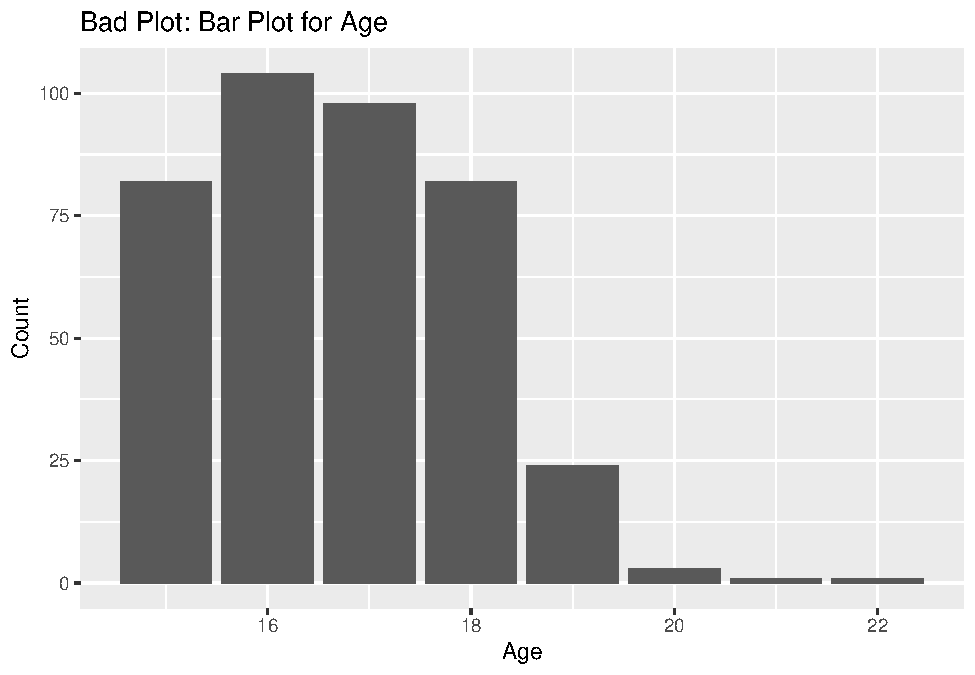
\includegraphics{figs/unnamed-chunk-4.pdf}

\begin{Shaded}
\begin{Highlighting}[]
\FunctionTok{ggplot}\NormalTok{(df, }\FunctionTok{aes}\NormalTok{(}\AttributeTok{x =} \StringTok{""}\NormalTok{, }\AttributeTok{fill =}\NormalTok{ Mjob)) }\SpecialCharTok{+}
  \FunctionTok{geom\_bar}\NormalTok{(}\AttributeTok{width =} \DecValTok{1}\NormalTok{) }\SpecialCharTok{+}
  \FunctionTok{coord\_polar}\NormalTok{(}\StringTok{"y"}\NormalTok{) }\SpecialCharTok{+}
  \FunctionTok{labs}\NormalTok{(}\AttributeTok{title =} \StringTok{"Bad Plot: Pie Chart for Mother\textquotesingle{}s Job"}\NormalTok{)}
\end{Highlighting}
\end{Shaded}

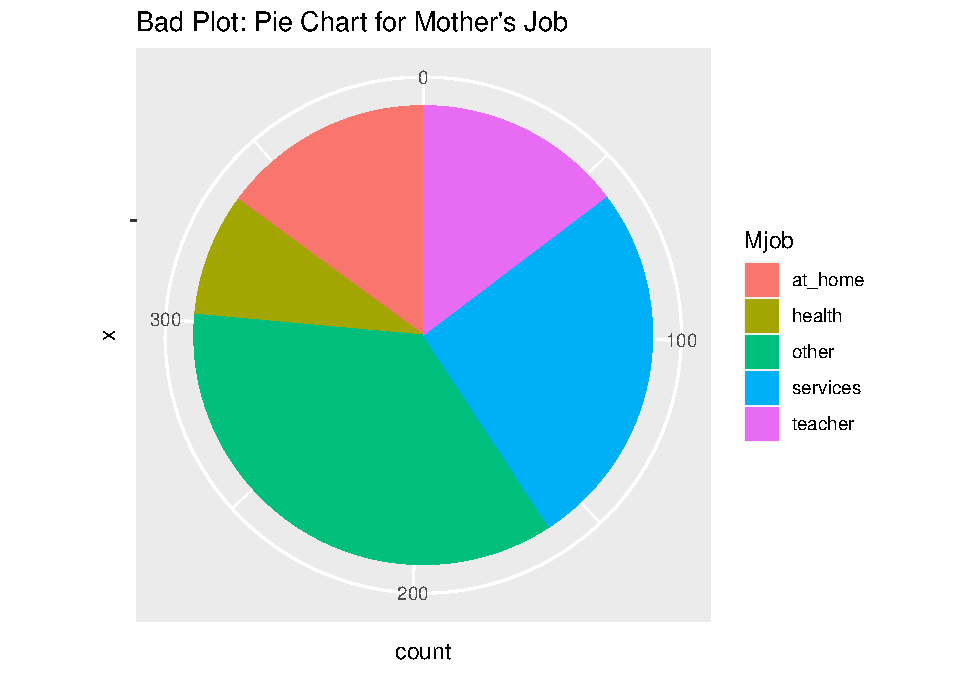
\includegraphics{figs/unnamed-chunk-5.pdf}

\section{Problem 3. Good Data
Visualization}\label{problem-3.-good-data-visualization}

\begin{Shaded}
\begin{Highlighting}[]
\FunctionTok{ggplot}\NormalTok{(df, }\FunctionTok{aes}\NormalTok{(}\AttributeTok{x =}\NormalTok{ age)) }\SpecialCharTok{+}
  \FunctionTok{geom\_histogram}\NormalTok{(}\AttributeTok{binwidth =} \DecValTok{1}\NormalTok{, }\AttributeTok{color =} \StringTok{"black"}\NormalTok{) }\SpecialCharTok{+}
  \FunctionTok{labs}\NormalTok{(}\AttributeTok{title =} \StringTok{"Correct Plot: Histogram for Age"}\NormalTok{, }\AttributeTok{x =} \StringTok{"Age"}\NormalTok{, }\AttributeTok{y =} \StringTok{"Frequency"}\NormalTok{)}
\end{Highlighting}
\end{Shaded}

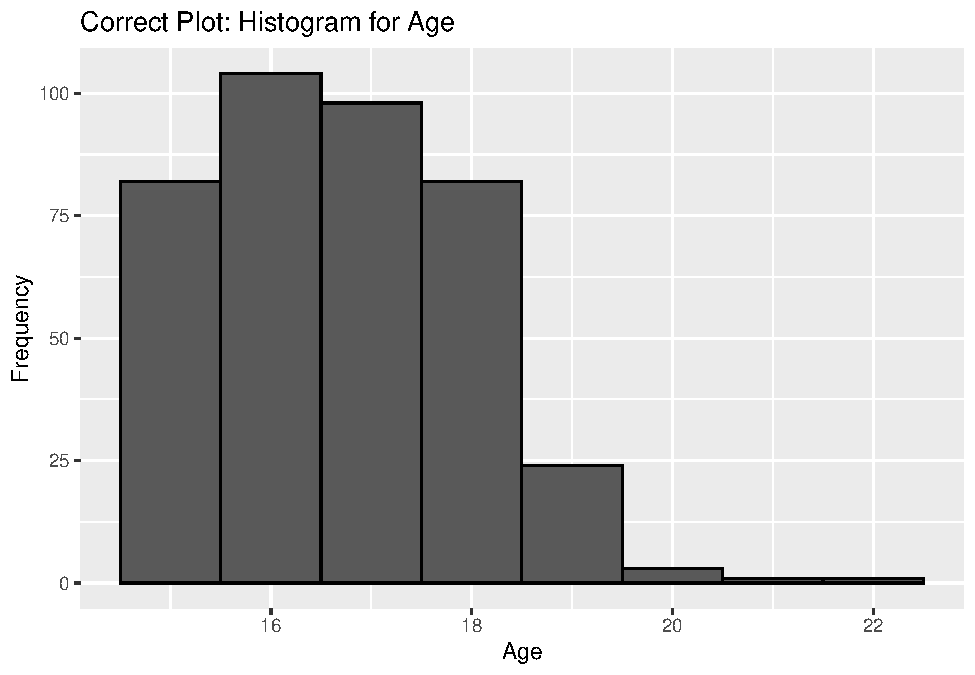
\includegraphics{figs/unnamed-chunk-6.pdf}

\begin{Shaded}
\begin{Highlighting}[]
\CommentTok{\# Correct plot: Bar plot for categorical variable (Mjob)}
\FunctionTok{ggplot}\NormalTok{(df, }\FunctionTok{aes}\NormalTok{(}\AttributeTok{x =}\NormalTok{ Mjob)) }\SpecialCharTok{+}
  \FunctionTok{geom\_bar}\NormalTok{(}\AttributeTok{fill =} \StringTok{"skyblue"}\NormalTok{, }\AttributeTok{color =} \StringTok{"black"}\NormalTok{) }\SpecialCharTok{+}
  \FunctionTok{labs}\NormalTok{(}\AttributeTok{title =} \StringTok{"Correct Plot: Bar Plot for Mother\textquotesingle{}s Job"}\NormalTok{, }\AttributeTok{x =} \StringTok{"Mother\textquotesingle{}s Job"}\NormalTok{, }\AttributeTok{y =} \StringTok{"Count"}\NormalTok{) }\SpecialCharTok{+}
  \FunctionTok{theme}\NormalTok{(}\AttributeTok{axis.text.x =} \FunctionTok{element\_text}\NormalTok{(}\AttributeTok{angle =} \DecValTok{45}\NormalTok{, }\AttributeTok{hjust =} \DecValTok{1}\NormalTok{))}
\end{Highlighting}
\end{Shaded}

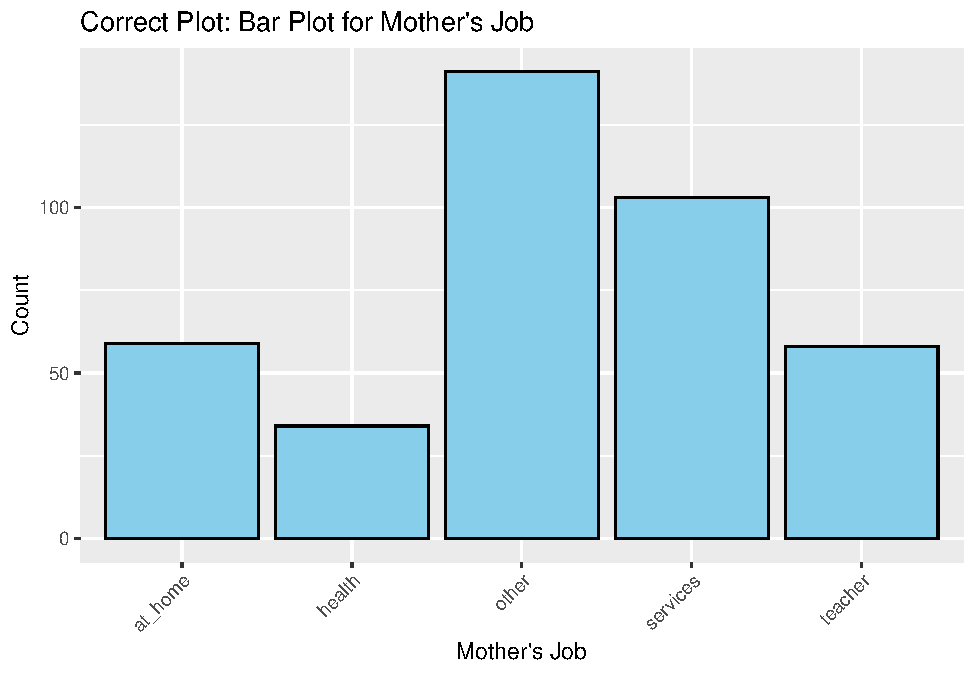
\includegraphics{figs/unnamed-chunk-7.pdf}

\section{Problem 4. Simple analysis}\label{problem-4.-simple-analysis}

TBD

\end{document}
